\documentclass[aspectratio=169, 22pt]{beamer}

\usepackage{amsmath}
\usepackage{slidedefs}
\usepackage{listings}

\title{Open-Source Software's Responsibility to Science}
\subtitle{}
\date{20th July 2018}
\author{Joel Nothman}

\usetheme[logobar]{usyd}

\titlegraphic{fig/title-slide}
\titlegraphicbackground{usydred}

\newcommand{\hl}{\textcolor{usydred}}
\newcommand{\ex}{\textcolor{usydblue}}
\newcommand{\issue}[1]{\href{https://github.com/scikit-learn/scikit-learn/issues/#1}{\##1}}

\newenvironment{sectionslide}
			{\subsection*{+}\begin{frame}[fragile,environment=sectionslide]\vfill\begin{center}\Large}
			{\end{center}\vfill\end{frame}}


\begin{document}

\titleslide

\section{Gatekeepers}

\begin{points}{Me in open source}
	\p Mostly contributed to popular Scientific Python libraries:\\
	scikit-learn, nltk, scipy.sparse, pandas, ipython, numpydoc
	\p Also information extraction evaluation (neleval), etc.
	\vfill
	\p Community service
	\p ``Volunteer software development''
	\p With thanks to our financial sponsors
	\vfill
	\p Caretakers aren't always founders
	\p Founders aren't always caretakers
\end{points}

\begin{centre}{Overheard at ICML}
	\parbox{\textwidth}{
		\Large
		\it
	Don't worry about how tricky it is to implement \ldots

	\vspace{2em}

	\raggedleft Someone will put it in Scikit-learn and you can just use it.
	}
\end{centre}

\begin{points}{Thoughts on an arrogant ML researcher}
	\p Scientists think software maintenance is no big deal
	\pause
	\vfill
	\p Science and engineering rely heavily on open-source infrastructure
	\p Popular tools become de-facto standards
	\vfill
	\p Most users are uncomfortable building their own tools
	\p Many will only use what's provided in a popular library
	\p Many will not inspect how it works on the inside
	\vfill
	\p Volunteer maintainers act as gatekeepers
\end{points}

\begin{points}{The power of the gatekeeper}
	\p decides \hl{which algorithms} are available
	\p decides how to ensure \hl{correctness} and stability
	\p decides how to \hl{name} or describe the algorithm
	\p decides whether to be \hl{faithful} to a published description
	\p decides on an \hl{API} that may facilitate good science/engineering
	\\
	\pause
	\vspace{2em}
	\hl{\bf OSS maintainers can enable or inhibit scientific best practices}
\end{points}

\begin{centre}{But you can't blame the gatekeeper}
	\begin{quote}
	THIS SOFTWARE IS PROVIDED BY THE COPYRIGHT HOLDERS AND CONTRIBUTORS \textbf{``AS IS''}
	AND ANY EXPRESS OR IMPLIED WARRANTIES, INCLUDING, BUT NOT LIMITED TO, THE
	IMPLIED WARRANTIES OF MERCHANTABILITY AND FITNESS FOR A PARTICULAR PURPOSE
	ARE DISCLAIMED.
	\end{quote}
\end{centre}


% TODO Talk about risks?

\begin{points}{This presentation is a series of examples}
	\p Risks to good science and engineering related to software design
	\vfill
	\p Some things we do to help science
	\p Some things we have changed to help science
	\p Some things we have yet to solve
	\vfill
	\p There's not a great deal of NLP in here \\
	but there's a lot of ML and software engineering in NLP\\
	(so I hope it is relevant, interesting and accessible)
\end{points}


\begin{points}{Scikit-learn preliminaries}
	\p An ecosystem of estimators
	\p Fit an estimator on some data, so that it can:
	\begin{itemize}
		\p describe the training data
		\p transform unseen data
		\p predict a target for unseen data
	\end{itemize}
	\p Data is usually a numeric matrix \verb|X| (samples $\times$ features)
	\p May provide a target vector or matrix \verb|y| at training time
	\begin{itemize}
		\p real valued for regression
		\p categories for multiclass classification
		\p multiple columns of binary targets for multilabel classification
	\end{itemize}
\end{points}

% TODO: introduce multiclass, multi-label
% TODO: introduce feature representations..?

\section{Names}

\begin{sectionslide}
	Methods and results and are indecipherable if researchers publish an inappropriate, or underspecified, algorithm name
\end{sectionslide}


% https://github.com/scikit-learn/scikit-learn/issues/9993
\begin{points}{A simple example of a bad name}
	\p \verb|sklearn.covariance.GraphLasso| for sparse inverse covariance estimation
	\p but \emph{Graph Lasso} is sparse \emph{regression} where the features lie on a graph
	\p the paper for covariance estimation named it \emph{Graphical Lasso}
	\pause
	\p[Solution] deprecate \verb|GraphLasso| and rename it \verb|GraphicalLasso|
\end{points}

\begin{points}{Tripping over hidden parameters}
	\p 
\verb|precision_score([`a',`a',`b',`b',`c'], [`a',`b',`b',`c',`c'])|
	\p For multi-class or multi-label, how should you average across classes?
	\begin{itemize}
\p $P_a = \frac{1}{1}$, $P_b = \frac{1}{2}$, $P_c = \frac{1}{2}$
\p average='micro' $\Rightarrow$ $\frac{3}{5}$
\p average='macro' $\Rightarrow$ $(1 + \frac{1}{2} + \frac{1}{2}) / 3 = \frac{2}{3}$
\p average='weighted' $\Rightarrow$ $(2\times1 + 2\times\frac{1}{2} + 1\times\frac{1}{2}) / 5 = \frac{7}{10}$
	\end{itemize}
	\p for a long time, prevalence-weighted macro average was the default
	\begin{itemize}
	\p[$\therefore$] papers say ``We achieved a precision of \dots''
	\end{itemize}
	\pause
\p[Solution] \verb|precision_score| raises an error if the data is not binary,\\
unless the user specifies \verb|average|. \\ \hfill \textbf{\hl{Use the API to force literacy \& awareness}}
\end{points}

\iffalse
\begin{points}{API convenience leads to inappropriate names}
	\p \verb|OneVsRestClassifier| does OvR:\\
	naively turns a multiclass problem into a series of binary classifications
	\p It also does \emph{binary relevance}:\\
	naively turns a multilabel problem into a series of binary classifications
	\p It chooses which mode depending on the shape of the input
	\p Convenient, but eventually the ambiguity creates problems
	\pause
	\p[Unsolved]
\end{points}
\fi

\begin{points}{What's in a name?}
	\p What makes an implementation of some named algorithm \hl{correct}?
	\vfill
	\p Faithful to a published research paper?
	\p Faithful to a reference implementation?
	\p Faithful to \emph{some} community of practice?
	\p Consistent with other components of our software library?
	\p Consistent with previous versions of the library?
\end{points}

\section{Surprises}

\begin{sectionslide}
	Experimenters report sub-optimal results\\
	because they assume our implementation is nicely behaved
\end{sectionslide}

\begin{points}{The fit you thought was finished}
	\p Many optimisations are iterative
	\p have criteria to test if it has converged on an optimum
	\p Predictions and inferences may be poor if parameters did not converge
	\pause
	\p[Solution] Warn if we did not detect convergence \\
	but if we have too many warnings, users ignore them\ldots
\end{points}

% Hidden surprises
%  - macro-average of only training set classes ????
\begin{points}{The words you didn't mean to stop}
	\p \verb|CountVectorizer| turns text into a term-document matrix
	\p can choose stop words: None, `english' or BYO
	\p `english' will remove \emph{system} (and used to remove \emph{computer})
	\p `english' will remove \emph{five}, \emph{six}, \emph{eight} but not \emph{seven}
	\p `english' will remove \emph{we have} but treat \emph{we've} as \emph{ve}
	\p This is documented nowhere.
	\p See my NLP-OSS paper with Hanmin Qin and Roman Yurchak
	\pause
	\p[Solution] Deprecate `english' 
	\pause and add another \hl{perfect} stop list \ldots
\end{points}

\begin{points}{The intercept you didn't mean to regularise}
	\p In Logistic Regression, we learn a weight vector $\mathbf{\beta}$
	\p and a bias term $\beta_0$ which corresponds to a feature $\mathbf{x}_0$ of all-1s
	\p Regularisation: minimise $\sqrt{\sum_i \beta_i^2}$ to ensure small weights as well as small loss 
	\p liblinear regularises $\beta_0$. You probably never want to do this.
	\p All our other linear estimators do not regularise the intercept.
	\pause
	\p[Sol'n 1] \verb|intercept_scaling|: also need to optimise $\mathbf{x}_0$'s fill value\\
	\pause
	\ldots but most users don't see/do this
	\p[Sol'n 2] Implement alternative optimisers, and deprecate liblinear as default LogisticRegression solver
\end{points}

\section{Sensibility}

\begin{sectionslide}
	\emph{Analysis of code on GitHub shows that people use default parameters when they shouldn't} \\
	\raggedleft Andreas M\"uller
\end{sectionslide}

\begin{plain}{Most users are lazy}
	\begin{columns}[t]\begin{column}{.65\textwidth}
		\vspace{-2em}
	\begin{itemize}
	\p Users don't explore alternatives
	\begin{itemize}
		\p alternative parameters values
		\p alternative software libraries
	\end{itemize}
	\p My students tend to use a \verb|CountVectorizer| even when they're counting non-words (e.g.\ synsets)
%%%	\p[Sol'n?] Replace \verb|CountVectorizer| with a text counter to encourage use of generic \verb|DictVectorizer|
	\p We try to provide sensible default parameters
	\end{itemize}
	\vfill
\end{column}
\begin{column}{.39\textwidth}
	\vspace*{-50pt}
	\fbox{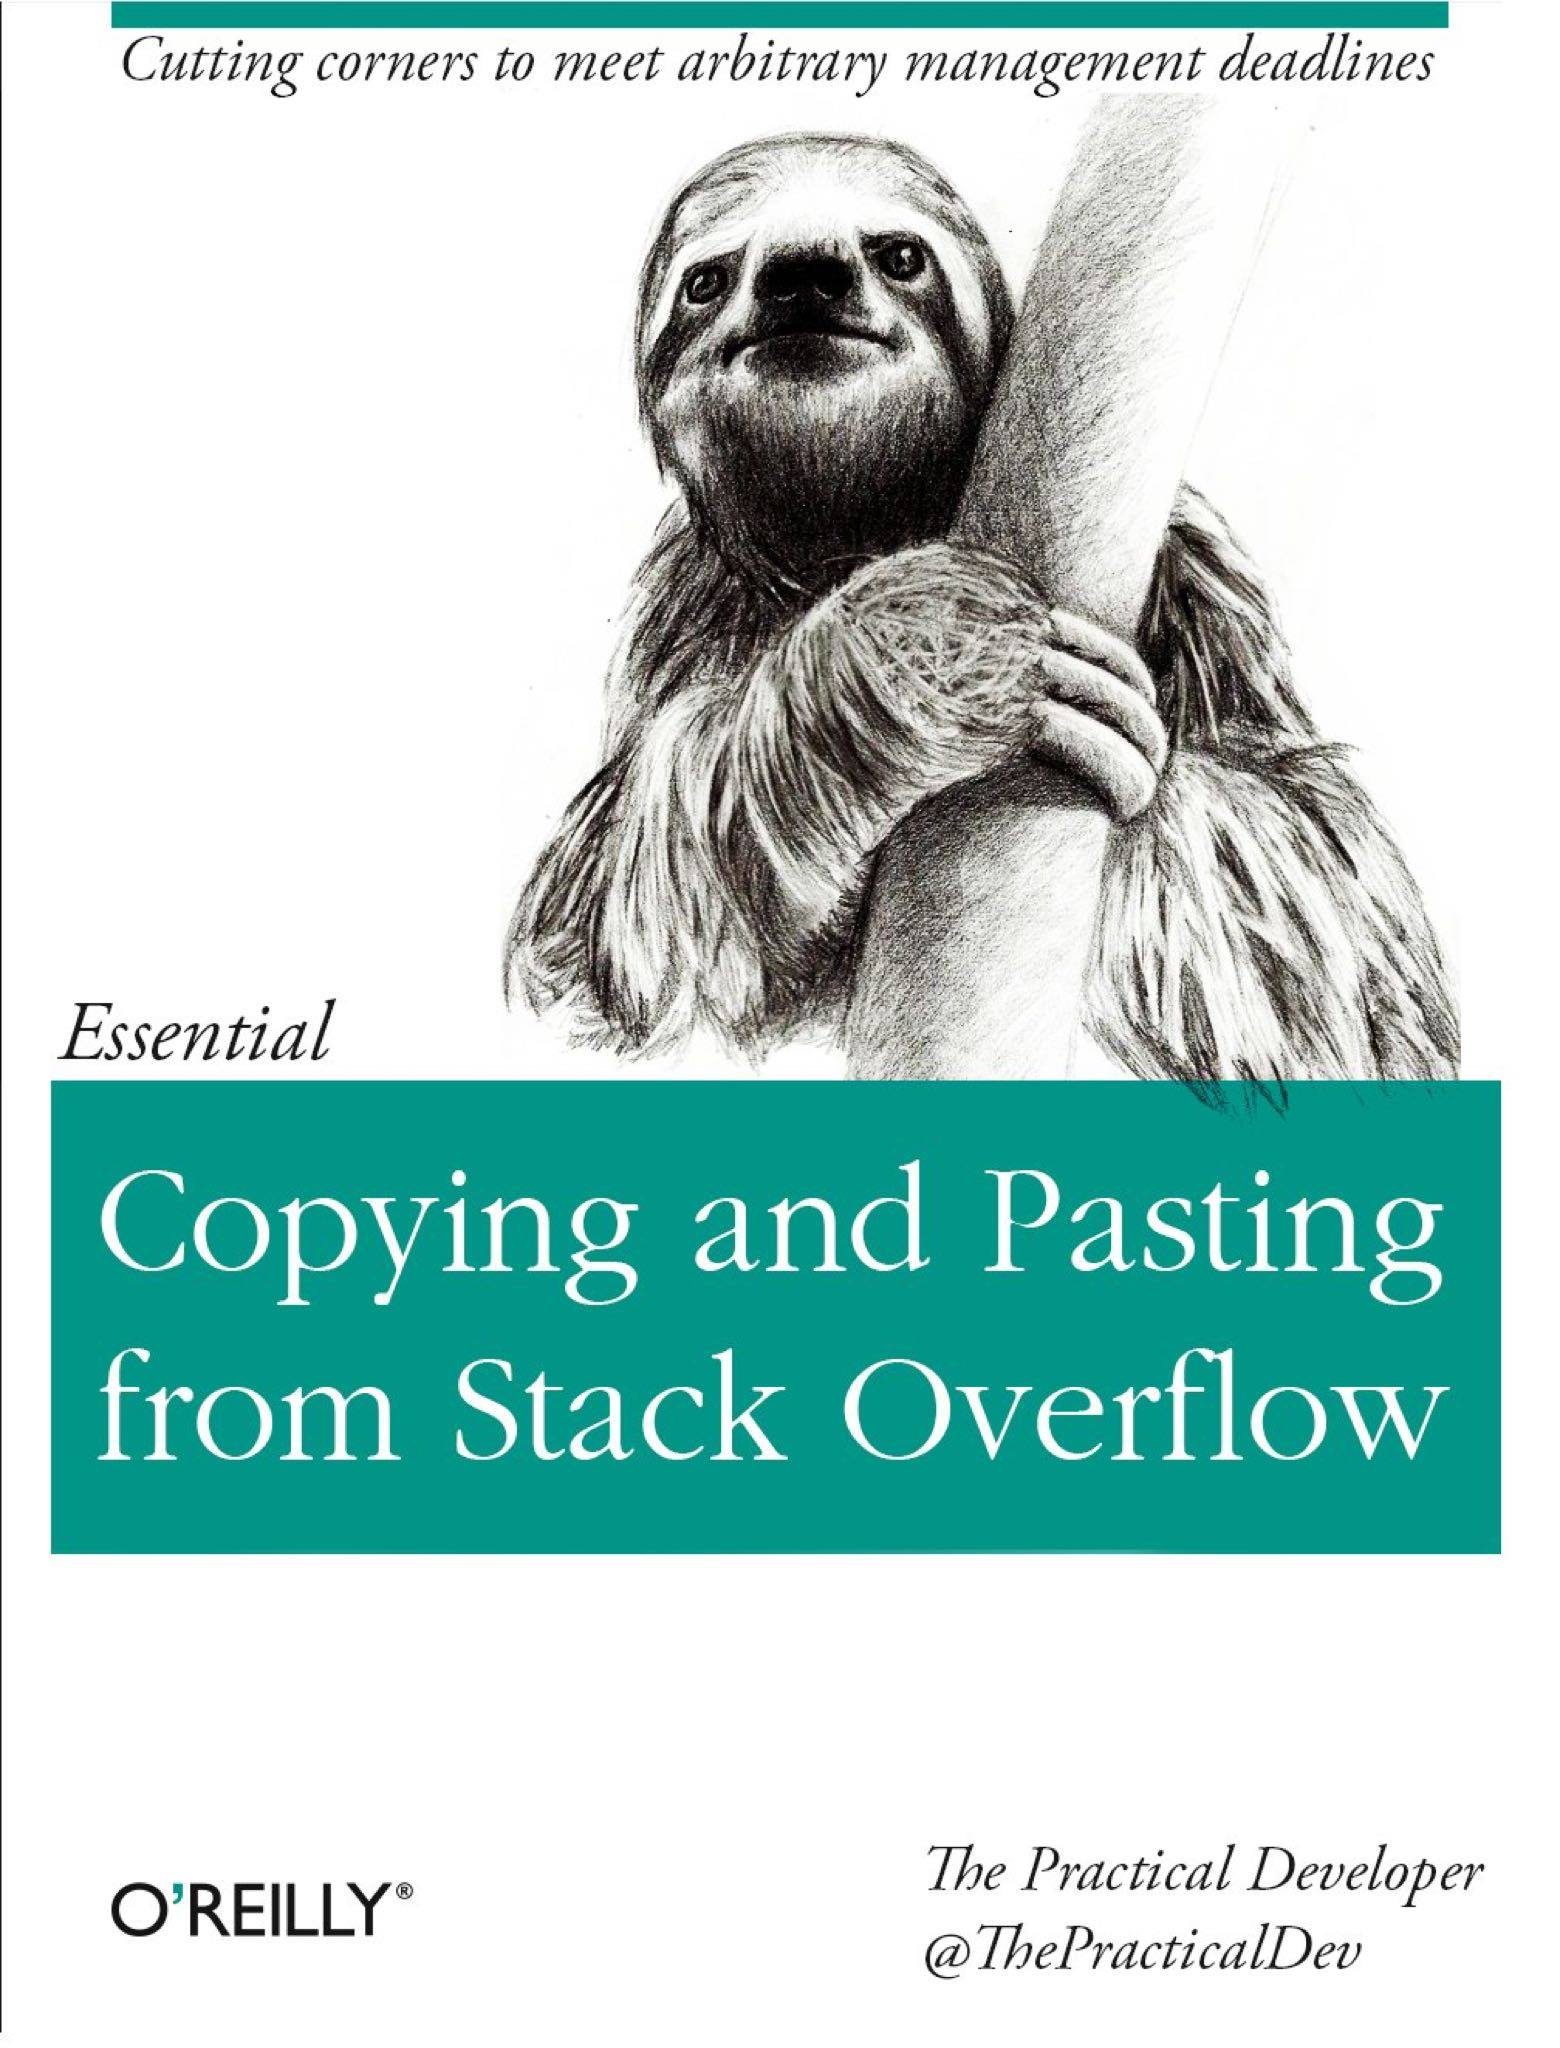
\includegraphics[width=\columnwidth]{fig/stackoverflow}}
\end{column}
\end{columns}
\end{plain}

\begin{points}{Sensible default fail}
	\p Ten-tree forests
	\p Three-fold cross validation
	\p ?? A tokeniser that splits on word-internal punctuation
%%%	\vfill
%%%	\p Contributors come and go
%%%	\p Sometimes we don't know why things are the way they are
\end{points}

\begin{points}{What makes a default value good?}
	\p Good defaults should give good predictive models and reliable statistics
	\p ? Good defaults should behave how users expect
	\begin{itemize}
			\p but different communities of practice
	\end{itemize}
	\p Good defaults should be invariant to:
	\begin{itemize}
			\p sample size (for stability in cross validation)
			\p number of features (for stability in model selection)
			\p ?feature scaling (for stability in different tasks/datasets)
	\end{itemize}
	\p Example:	finding a good default $\gamma$ for an RBF kernel (\issue{779}, \issue{10331})
	% TODO: the scaling of regularization coefficients might be more relevant, but is hard to express: https://github.com/scikit-learn/scikit-learn/issues/10164
\end{points}

\begin{points}{Good parametrisation}
	\p We choose the defaults, but also how parameters are expressed
	\p (and whether they can be changed at all)
	\vfill
	\p Should number of nearest neighbors be specified as:
	\begin{itemize}
		\p an absolute value (e.g.\ 10)?
		\p a proportion of training samples (e.g.\ 2\%)?
		\p an arbitrary function of training data shape?
	\end{itemize}
	\vfill
	\p Algorithms and optimisation research often don't report on this
\end{points}

% FIXME: find a better title
\section{Misdirection} % or breakage

% Other peoples' examples:
% • Providing P-values means people will misinterpret them
% • Restricting identifiers to 30 chars (Oracle) forces users to write immemorable abbreviations
% • Encouraging users to write neat code by the one right way to do something being clear (something numpy and pandas fail at)

\begin{sectionslide}
Scientific software should make it easy for users to do good science.
\end{sectionslide}
% By misuse I don't mean dishonesty

\begin{plain}{Have you ever tried to de-tokenise the Penn TreeBank?}
	\begin{itemize}
	\p PTB is delivered with each token POS tagged or bracketed
	\p We wanted to know how paragraph structure, etc.\ informed parsing
	\p The source text before tokenisation is available
	\p An easy case:
	\end{itemize}
	% XXX: had trouble using \only, so implementing it manually
	\begin{columns}\hspace{.05\textwidth}\begin{column}{.3\textwidth}
		{		\color{usydblue}
\verb|[ Imports/NNS ]|\\
\verb|were/VBD at/IN|\\
\verb|[ $/$ 50.38/CD billion/CD ]|\\
\verb|,/, up/RB|\\
\verb|[ 19/CD %/NN ]|\\
\verb|./.|}
\end{column}
%%%\begin{column}{.05\textwidth}\begin{center}to\end{center}\end{column}
	\begin{column}{.3\textwidth}
		\ex{Imports were at \$50.38 billion, up 19\%.}\\
		\vspace*{1em}
	{\small
	\begin{tabular}{ll}
		Imports & 1--7 \\
		were & 9--12 \\
		at & 14--15 \\
		\$ & 16--16 \\
		50.38 & 17--21 \\
	\end{tabular}
	}
\end{column}\end{columns}
\end{plain}

\begin{frame}\frametitle{Have you ever tried to de-tokenise the Penn TreeBank?}
\newcommand\p\item
	\begin{itemize}
	\p PTB is delivered with each token POS tagged or bracketed
	\p We wanted to know how paragraph structure, etc.\ informed parsing
	\p The source text before tokenisation is available
	\p[$\Rightarrow$] \hl{alignment hell} due to typos corrected/inserted, reorderings, missed text, etc.
	\vfill
	\p Hindsight: delivering annotations on tokenised text is a bad idea
	\p It restricts what you can do with it later
	\p NLP software should always provide stand-off markup
	\p Or store the whitespace/non-token data as spaCy does
	\end{itemize}
\end{frame}

\begin{plain}{Avoiding leakage in cross validation}
% Leakage
%  - at some point you need to roll your own
%  - when you roll your own you introduce errors
%  - Making sure imputers are inductive
	\begin{columns}[t]\begin{column}{0.1\textwidth}Bad\end{column}\begin{column}{.9\textwidth}
\verb|X_preprocessed = preprocessor.fit_transform(X)|\\
\verb|result = cross_validate(classifier, X_preprocessed, y)|

	\vspace{1em}
Test data statistics \hl{leak} into preprocessing\\
	$\Rightarrow$ inflated cross validation results
	\end{column}\end{columns}
	\vspace{1em}

	\begin{columns}[t]\begin{column}{0.1\textwidth}Good\end{column}\begin{column}{.9\textwidth}
\verb|pipeline = make_pipeline(preprocessor, classifier)|\\
\verb|result = cross_validate(pipeline, X, y)|
	\end{column}\end{columns}

	\vfill
	\pause
	\begin{itemize}
			\p[Solution] De-emphasise \verb|fit_transform|.\\
			And make sure \verb|Pipeline| works with everything;\\
			and make sure \verb|cross_validate| works with everything.
	\end{itemize}
\end{plain}

% Cross_val_predict :(

\section{Collaborate}

{%
\setbeamertemplate{background}{\parbox{\paperwidth}{\vspace{2mm}\raggedleft
\includegraphics[height=\paperheight]{fig/unicorn-2007266_1280}}}
%%%\begin{points}{Maintainers need feedback from scientists}
\begin{sectionslide}
	Maintainers of large projects\\can't be experts in \emph{all} the things they maintain
\end{sectionslide}
%%%\end{points}
}

\begin{points}{Scientists can (and do) help us:}
	\p make sure the implementation matches the name
	\p make users aware of or avoid unexpected behaviour
	\p parametrise algorithms and set defaults helpfully
	\p understand how our design choices lead to flawed experiments
	\vfill
	\raggedleft
	\hl{\bf Users trust popular OSS.}\\
	\hl{\bf Thank you for helping us make OSS trustworthy.}
\end{points}
% Scientists helping out
%  - reporting issues
%     - not just errors or wishes
%  - helping to develop MICEImputer
%  - maintainers help by setting a standard of quality assurance


% Related work: The Architecture of Open Source Applications: http://aosabook.org/en/index.html

\end{document}
